\documentclass{beamer}
% * <nuevecuervos@gmail.com> 2017-11-10T23:57:23.576Z:
%
% ^.
\usetheme{Stockton}
\usepackage{tikz}
\usepackage{tkz-berge}
\usepackage{pgf}
\usepackage{amsmath,amssymb}
\usepackage{graphicx}
\usepackage{verbatim}
\usepackage{subcaption}
\usepackage{multirow}
%\usepackage{ctable} 
\usepackage{geometry}
\usepackage{xcolor}
\usepackage{color}
%\usepackage{media9}
\usepackage{movie15}
%\usepackage{animate,media9,movie15}
\usepackage{wrapfig}
%\usepackage{multimedia}
\usepackage{hyperref}
\usetikzlibrary{shapes.geometric,arrows}

\addtobeamertemplate{navigation symbols}{}{%
    \usebeamerfont{footline}%
    \usebeamercolor[fg]{footline}%
    \hspace{1em}%
    \insertframenumber/\inserttotalframenumber
}


\setbeamercovered{transparent}
\title[Predicting Atomic Scale Fracture in Silica-Based Glasses]{Graph Theoretic Machine Learning Approaches to Predict Atomic Scale Fracture in Silica-Based Glasses}
\subtitle[SNL]{Sandia National Laboratories}



\author[S. Cheng, Y. Kim, A. Lawrence, C. Oroz]{\textbf{Students:} Shu Cheng, Yuri Kim, Adam Lawrence, Corina Oroz \textbf{Faculty Advisor:} Allon Percus \\ \textbf{Liaisons:} Mark Wilson, Thomas Hardin}
\institute[CGU]{Claremont Graduate University}

\date{November 20, 2019}

\begin{document}
\frame{\titlepage}

\section{Introduction}
\subsection{Background}
\frame
{
\frametitle{Background}
\begin{block}{}
A fundamental engineering challenge surrounding brittle materials is predicting failure. This involves predicting where fractures \textbf{nucleate} as well as how these fractures \textbf{propagate}.
\newline
\newline
Researchers at Sandia National Laboratories have used Molecular Dynamics (MD) simulations to model the effects that cause nucleation and growth, but this is computationally intensive.
\end{block}
}

%%%%%%%%%%%%%%%%%%%%%%%%%%%%%%%%%%%%%%%%%%%%%%%%%%%%%%%%%%%%%%%%%%%%%%%%%%%%%%%%%%%%%%%%%

\frame{
\frametitle{ Sandia National Laboratories}
\begin{minipage}[0.2\textheight]{\textwidth}
\begin{columns}[T]
    \begin{column}{0.5\textwidth}
    
  \begin{block}{}
    \textbf{Sandia's Interest:} Brittle materials are used throughout the stockpile. Examples include headers, electronic connectors, etc. 
    \newline
    \newline
    \textbf{Challenge:} Make reliability predictions for components containing brittle materials. 
  \end{block}
    \end{column}
    
    \begin{column}{0.5\textwidth}
    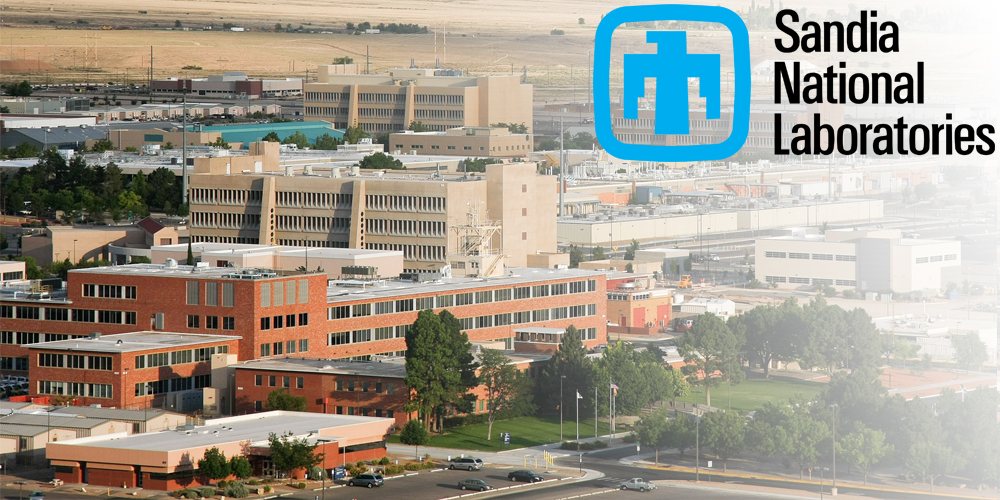
\includegraphics[width=5.5cm]{images/sandia.jpg}
    \end{column}
\end{columns}
\end{minipage}
}

%%%%%%%%%%%%%%%%%%%%%%%%%%%%%%%%%%%%%%%%%%%%%%%%%%%%%%%%%%%%%%%%%%%%%%%%%%%%%%%%%%%%%%%%%

\frame
{
\frametitle{Motivation}
\begin{block}{}
The clinic aims to develop a model that rapidly predicts where fractures will form silica-based glasses. We consider different environmental conditions including different boundary properties exposure to water.
\newline
\newline
By creating a graph theoretic description of the material we will train a supervised \textbf{Machine Learning (ML)} algorithm on MD simulation data.
\end{block}
}

%%%%%%%%%%%%%%%%%%%%%%%%%%%%%%%%%%%%%%%%%%%%%%%%%%%%%%%%%%%%%%%%%%%%%%%%%%%%%%%%%%%%%%%%%

\frame
{
\frametitle{Physical Structure}
   \begin{columns}
    	\begin{column}{.5\textwidth}
			\begin{figure}[!b]
    \centering
    \noindent
\begin{tikzpicture}[scale=.65]
\coordinate (A) at (-0.5,0.5,0); % Left back O 
\coordinate (B) at (2,0.5,4.5); % Left front O  
\coordinate (C) at (6,0.5,0); % Right back O
\coordinate (D) at (6.5,0.5,5); % Right front O 
\coordinate (E) at (3.75,1,2.5); % Bridging Oxygen 
\coordinate (F) at (5.5,1.5,2.5); % Right Si
\coordinate (G) at (2,1.5,2.5); % Left Si 
\coordinate (H) at (1.5,3,2.5); % Left top O 
\coordinate (I) at (6,3,2.5); % Right Top O

%connections from left Si
\draw [very thick] (G) -- (A);
\draw [very thick] (G) -- (B);
\draw [very thick] (G) -- (H);
\draw [very thick] (G) -- (E);

%connections from Right Si 
\draw [very thick] (F) -- (C);
\draw [very thick] (F) -- (D);
\draw [very thick] (F) -- (I);
\draw [very thick] (F) -- (E);

%dashed lines between Oxygen. This can be removed but it was in literature. 
\draw[gray,dashed] (A) -- (H);
\draw[gray,dashed] (H) -- (B);
\draw[gray,dashed] (B) -- (A);
\draw[gray,dashed] (A) -- (E);
\draw[gray,dashed] (H) -- (E);
\draw[gray,dashed] (B) -- (E);

\draw[gray,dashed] (I) -- (C);
\draw[gray,dashed] (C) -- (D);
\draw[gray,dashed] (D) -- (I);
\draw[gray,dashed] (I) -- (E);
\draw[gray,dashed] (D) -- (E);                                                
\draw[gray,dashed] (C) -- (E);  

%place non-atom cube corners
\shadedraw [ball color= white] (A) circle (0.3cm);
\shadedraw [ball color= white] (B) circle (0.3cm);
\shadedraw [ball color= white] (C) circle (0.3cm);
\shadedraw [ball color= white] (D) circle (0.3cm);
\shadedraw [ball color= white] (E) circle (0.3cm);
\shadedraw [ball color= red] (F) circle (0.20cm);
\shadedraw [ball color= red] (G) circle (0.20cm);
\shadedraw [ball color= white] (H) circle (0.3cm);
\shadedraw [ball color= white] (I) circle (0.3cm);
\end{tikzpicture}
    %\caption{Two silicon atoms (red)\\with surrounding oxygen atoms (grey) in tetrahedral configuration. A bridging %oxygen is at the center.}
    
    \label{fig:tetrahedra}
\end{figure}

    {\bf SiO$_\mathbf{2}$}: Two silicon atoms (red)\\with surrounding oxygen atoms (grey) in tetrahedral configuration. A bridging oxygen is at the center.
    
		\end{column}
   		\begin{column}{.6\textwidth}
        \begin{block}{}
		\begin{itemize} 
        \item Nucleation is related to atomic-scale defects or chemical bond weakness in the glass
		\begin{itemize} 
        \item The relationship between atomic structure and fracture behavior is complex 
		\end{itemize}
        \item Nucleation and propagation depend more on subtle characteristics of the local structure surrounding an atom\\
    \end{itemize}
    \end{block}
		\end{column}
	\end{columns}
}

%%%%%%%%%%%%%%%%%%%%%%%%%%%%%%%%%%%%%%%%%%%%%%%%%%%%%%%%%%%%%%%%%%%%%%%%%%%%%%%%%%%%%%%%%

\subsection{Previous Work}
\frame
{\frametitle{Molecular Dynamics Simulations}
\begin{block}{}
Molecular dynamics (MD) methods simulate the system at the nanoscale and model the individual chemical and physical interactions taking place in the material.
\newline
\newline
These simulations have successfully predicted a wide range of detailed
properties that cannot be obtained with continuum methods, and that are
consistent with experimental observations.
\end{block}
}

%%%%%%%%%%%%%%%%%%%%%%%%%%%%%%%%%%%%%%%%%%%%%%%%%%%%%%%%%%%%%%%%%%%%%%%%%%%%%%%%%%%%%%%%%

\frame
{
\frametitle{LAMMPS}
\begin{block}{} 

Sandia has developed molecular dynamics simulation software Large-scale Atomic/Molecular Massively Parallel Simulator.

Simulations are generated using the LAMMPS code. Each LAMMPS run simulates a sample of SiO2 containing approximately 70,000 atoms.
\end{block}
}

%%%%%%%%%%%%%%%%%%%%%%%%%%%%%%%%%%%%%%%%%%%%%%%%%%%%%%%%%%%%%%%%%%%%%%%%%%%%%%%%%%%%%%%%%





\subsection{Math Clinic Goals}
\frame
{\frametitle{Objective}
\begin{block}{}
\begin{itemize}
    \item Develop supervised learning methods, trained on MD simulation data, that generate rapid predictions of where and when atomic-scale fractures occur in samples of silicate glasses under stress. 

\item Generate predictions under multiple environmental conditions, validate on existing MD simulation results. 

\item Relate predictions to specific features characterizing local atomic structure.

\item Provide new insight into how local structure leads to fracture and failure.
\end{itemize}
\end{block}
}

\frame
{\frametitle{Goals}
\begin{block}{}

\textbf{Goal 1:} Predict fracture nucleation events.
\newline
\newline

\textbf{Goal 2:} Predict fracture propagation.

\end{block}
}
\section{Model}
%%%%%%%%%%%%%%%%%%%%%%%%%%%%%%%%%%%%%%%%%%%%%%%%%%%%%%%%%%%%%%%%%%%%%%%%%%%%%%%%%%%%%%%%%%%%%%%%%%%%%%%%%%
\subsection{Data}
\frame
{
\frametitle{Data}
\begin{block}{}
\begin{itemize}
    \item
Sandia has provided MD simulation results which we will use as training data for our ML models. 
\end{itemize}
\end{block}

\begin{block}{}
\begin{itemize}
    \item Two types of boundary conditions for simulations:
    \begin{itemize}
        \item Fully Periodic
        \item Free Surfaces
    \end{itemize}
\end{itemize}
\end{block}
}
%%%%%%%%%%%%%%%%%%%%%%%%%%%%%%%%%%%%%%%%%%%%%%%%%%%%%%%%%%%%%%%%%%%%%%%%%%%%%%%%%%%%%%%%%%%%%%%%%%%%%%%%%%
\frame
{
\frametitle{Descriptors}
\begin{block}{}
Data includes descriptors such as:
\begin{itemize}
    \item $x, y, z$ coordinates for each atom
    \item charge
    \item stress tensor
    \item bond connectivity
    \item newly formed/broken bonds
    \item Coordination number
    \item Number of bridging oxygens
    \item Volume surrounding atom
\end{itemize}
\end{block}
}
%%%%%%%%%%%%%%%%%%%%%%%%%%%%%%%%%%%%%%%%%%%%%%%%%%%%%%%%%%%%%%%%%%%%%%%%%%%%%%%%%%%%%%%%%%%%%%%%%%%%%%%%%%
\subsection{Representations}
\frame{
\frametitle{Representations}

\begin{minipage}[0.2\textheight]{\textwidth}
\begin{columns}[T]
    \begin{column}{0.5\textwidth}
    \vspace{2em}
    To achieve our goals, we will use the following representations to build the machine learning model:
    \begin{itemize}
    \item Graph Representations
    \item Feature Description
    \begin{itemize}
        \item Local Topological Feature
        \item Global Topological Feature
        \item Physical Feature
    \end{itemize}
    \item Extracting Ground Truth
    \end{itemize}
    \end{column}
    
    \begin{column}{0.5\textwidth}
    \vspace{2em}
    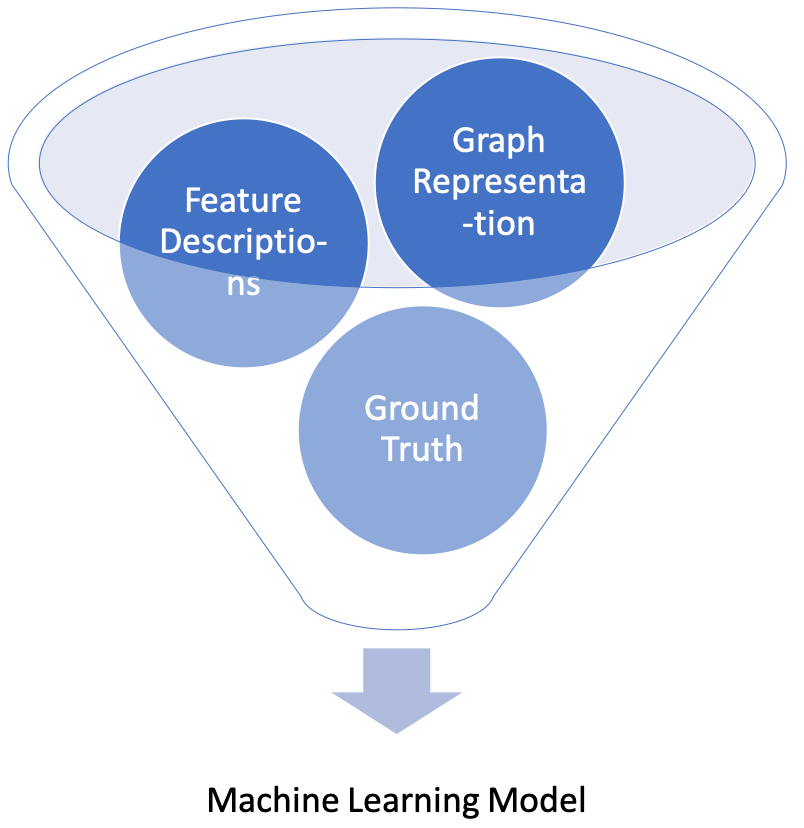
\includegraphics[width=5.5cm]{images/rep.png}
    \end{column}
\end{columns}
\end{minipage}
}


%%%%%%%%%%%%%%%%%%%%%%%%%%%%%%%%%%%%%%%%%%%%%%%%%%%%%%%%%%%%%%%%%%%%%%%%%%%%%%%%%%%%%%%%%%%%%%%%%%%%%%%%%%


\begin{frame}[t]{Graph Representations}
We propose three possible graph representations $G(t)=(V(t),E(t))$, where
$V(t)$ and $E(t)$ represent the set of vertices and edges at time $t$, respectively.

 \begin{columns}[t]
 
   \column{0.3\textwidth}
   \begin{block}{Basic Graph}
   \begin{itemize}
   \begin{footnotesize}
       \item $V$: Si, O atoms
       \item $E$: Chemical bond between atoms
    \end{footnotesize}
    \end{itemize}
    \begin{figure}
	    \centering
        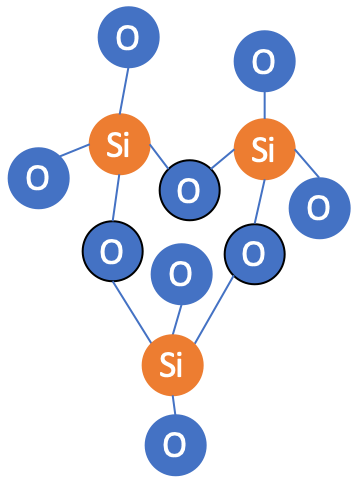
\includegraphics[width=.5\textwidth]{images/basic.png}
	\end{figure}
   \end{block}
   
   \column{0.3\textwidth}
   \begin{block}{Reduced Graph}
   \begin{itemize}
   \begin{footnotesize}
       \item $V$: Si atoms
       \item $E$: Bridging oxygens
    \end{footnotesize}
   \end{itemize}
    \begin{figure}
	    \centering
        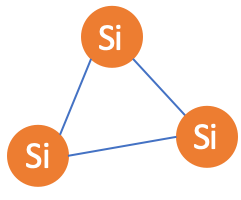
\includegraphics[width=.5\textwidth]{images/reduced.png}
	\end{figure}
   \end{block}
   
   \column{0.3\textwidth}
   \begin{block}{Topological Graph}
   \begin{itemize}
   \begin{footnotesize}
       \item $V$: Rings (closed paths)
       \item $E$: Bridging oxygen
    \end{footnotesize}
   \end{itemize}
    \begin{figure}
	    \centering
        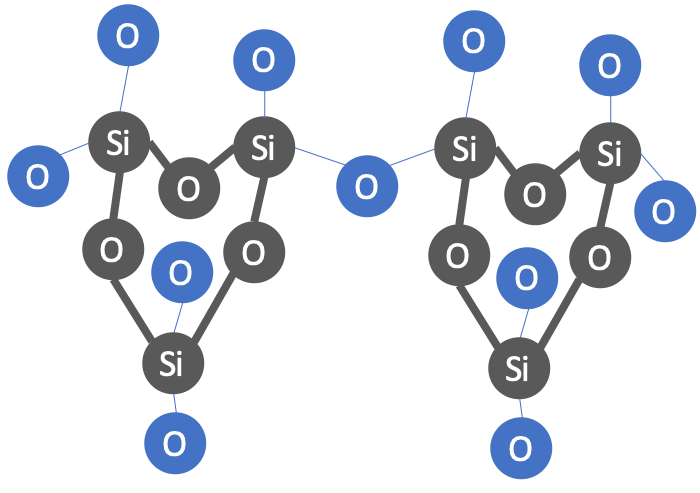
\includegraphics[width=.5\textwidth]{images/ring.png}
	\end{figure}   
   
   
   \end{block}
   
 \end{columns}
\end{frame}

%%%%%%%%%%%%%%%%%%%%%%%%%%%%%%%%%%%%%%%%%%%%%%%%%%%%%%%%%%%%%%%%%%%%%%%%%%%%%%%%%%%%%%%%%%%%%%%%%%%%%%%%%%
\frame
{\frametitle{Feature Description}
\begin{block}{}
\begin{itemize}
    \item Local Topological Features
    \item Global Topological Features
    \item Physical Features
\end{itemize}

\end{block}
}

%%%%%%%%%%%%%%%%%%%%%%%%%%%%%%%%%%%%%%%%%%%%%%%%%%%%%%%%%%%%%%%%%%%%%%%%%%%%%%%%%%%%%%%%%%%%%%%%%%%%%%%%%%
\frame{
\frametitle{Example of Local Topological Features}
\begin{block}{}
\textbf{Number of Bridging Oxygens:} In a Q$_n$ unit, an Si atom is surrounded by $n$ bridging O atoms, each forming an Si–O–Si group. The value of $n$ supplies crucial network connectivity information.
\begin{itemize}
    \item The number of bridging oxygens is equivalent to the degree of a vertex
    \item ML algorithms benefit from having bridging oxygens as an explicit feature
\end{itemize}
\end{block}

%\begin{block}{}
%k-th neighbor quantities. %See SOW
%\end{block}
}
%%%%%%%%%%%%%%%%%%%%%%%%%%%%%%%%%%%%%%%%%%%%%%%%%%%%%%%%%%%%%%%%%%%%%%%%%%%%%%%%%%%%%%%%%%%%%%%%%%%%%%%%%

\frame{
\frametitle{Example of Global Topological Features}

\begin{minipage}[0.2\textheight]{\textwidth}
\begin{columns}
    \begin{column}{0.5\textwidth}
   \textbf{Centrality Measures:}
quantify importance of an atom, relative to the rest of the network.

\bigskip

\begin{itemize}
    \item \textbf{Eigenvector Centrality}: High degree $\neq$ central role
    \item \textbf{Betweenness Centrality}: reflects node's importance in communication across graph
    \end{itemize}
    \end{column}
    
    \begin{column}{0.5\textwidth}
    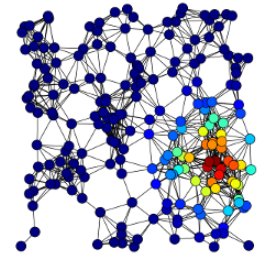
\includegraphics[width=5.5cm]{images/centrality.png}
    \end{column}
\end{columns}
\end{minipage}
}

%%%%%%%%%%%%%%%%%%%%%%%%%%%%%%%%%%%%%%%%%%%%%%%%%%%%%%%%%%%%%%%%%%%%%%%%%%%%%%%%%%%%%%%%%%%%%%%%%%%%%%%%%%

\frame
{
\frametitle{Example of Physical Features}


\begin{minipage}[0.2\textheight]{\textwidth}
\begin{columns}
    \begin{column}{0.6\textwidth}
    \begin{itemize}
    \item The \textbf{Voronoi cell volume, $v_i$}, is a local density measure. It measures how large the empty space is surrounding an atom $i$.
    \item Standardized cell volume, $\hat{v_i}$, can help filter out the affine displacement introduced by pulling the glass uni-axially.
    \newline
    $$\hat{v_i} = \frac{(v_i - \mu_v)}{\sigma_v}$$
    \newline
    \end{itemize}
    \end{column}
    
    \begin{column}{0.5\textwidth}
%    \vspace{4em}
    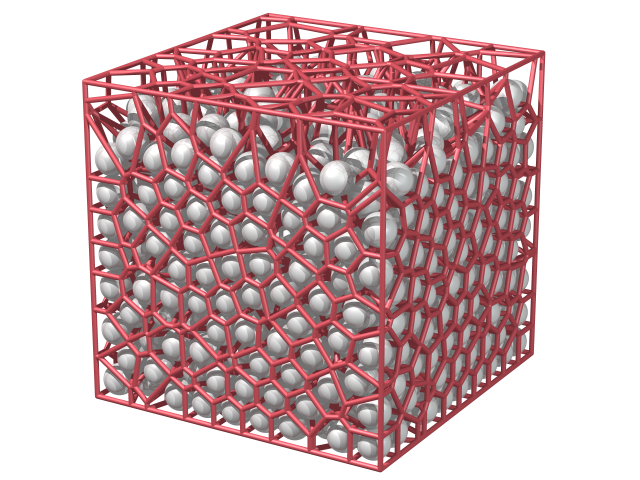
\includegraphics[width=5.5cm]{images/voronoi.png}
    \end{column}
\end{columns}
\end{minipage}
}

%%%%%%%%%%%%%%%%%%%%%%%%%%%%%%%%%%%%%%%%%%%%%%%%%%%%%%%%%%%%%%%%%%%%%%%%%%%%%%%%%%%%%%%%%%%%%%%%%%%%%%%%%%
\frame{

\frametitle{Extracting Ground Truth}

\begin{minipage}[0.2\textheight]{\textwidth}
\begin{columns}[T]
    \begin{column}{0.5\textwidth}
    
    \begin{itemize}
    \begin{footnotesize}
    \item 
    If $\hat{v_i} = \frac{(v_i - \mu_v)}{\sigma_v}$ exceeds a certain threshold, then atom $i$ is defined as part of a nucleation event. We define ground truth label as:
    $$
    y_i = \begin{cases}
      0 & \text{if }{\hat{v_i} \le 3} \\
      1 & \text{if }{\hat{v_i} \ge 3} \\
    \end{cases} 
    $$
    %%%%%%ground truth%%%%%%
    \item A K-nearest-neighbors algorithm will be applied to label those false-negative atoms.
    \end{footnotesize}  
    \end{itemize}
    \end{column}
    
    \begin{column}{0.5\textwidth}
    \vspace{3em}
    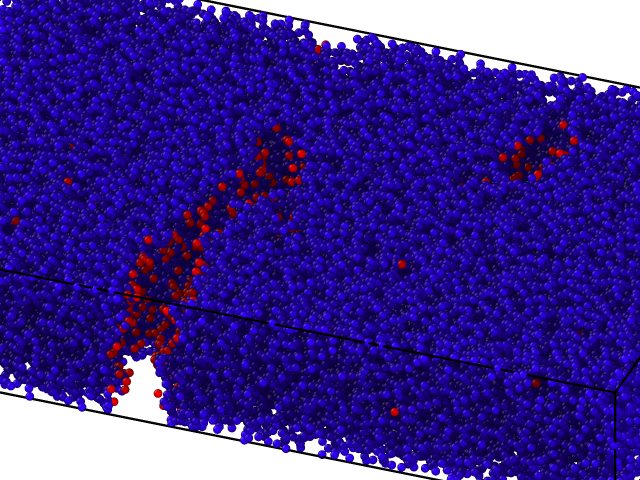
\includegraphics[width=5.5cm]{images/face.png}
    \end{column}
\end{columns}
\end{minipage}
}

%%%%%%%%%%%%%%%%%%%%%%%%%%%%%%%%%%%%%%%%%%%%%%%%%%%%%%%%%%%%%%%%%%%%%%%%%%%%%%%%%%%%%%%%%%%%%%%%%%%%%%%%%%
\subsection{Machine Learning}
\frame{
\frametitle{Machine Learning Methods}

\begin{block}{}
Objective is to produce surrogate model of MD simulations using supervised learning.

\begin{itemize}
    \item Use ensemble-based methods such as {\bf random forest} (RF) to predict nucleation at fixed future time step, given $t=0$ feature values.
    \item Use {\bf recurrent neural networks} (RNN) to learn dynamics of fracture propagation.
\end{itemize}
\end{block}
}

%%%%%%%%%%%%%%%%%%%%%%%%%%%%%%%%%%%%%%%%%%%%%%%%%%%%%%%%%%%%%%%%%%%%%%%%%%%%%%%%%%%%%%%%%%%%%%%%%%%%%%%%%%


\frame{
\frametitle{Ensemble methods}

{\bf Ensemble-based methods} predict atom labels by combining predictions from multiple estimators, learned from training data.

\medskip

\begin{block}{}

\begin{itemize}
    \item Bagging: {\bf random forest}.
    \begin{itemize}
        \item Estimators are decision trees constructed based on feature subsets drawn randomly with replacement.
        \item Labels determined by majority vote among decision trees.
    \end{itemize}
    
    \medskip
    
    \item Boosting: {\bf adaboost}.
    \begin{itemize}
        \item Estimators are classifiers based on individual features.
        \item Labels determined by weighted sum of classifier outputs, 
        weights updated successively to improve prediction accuracy.
    \end{itemize}
\end{itemize}
\end{block}
}
%%%%%%%%%%%%%%%%%%%%%%%%%%%%%%%%%%%%%%%%%%%%%%%%%%%%%%%%%%%%%%%%%%%%%%%%%%%%%%%%%%%%%%%%%%%%%%%%%%%%%%%%%%

\frame{
\frametitle{Recurrent Neural Networks}

RNN trains on an entire time series, learning dynamics of a process which it stores using a ``memory'' of internal states.

\begin{center}
\begin{figure}[!b]

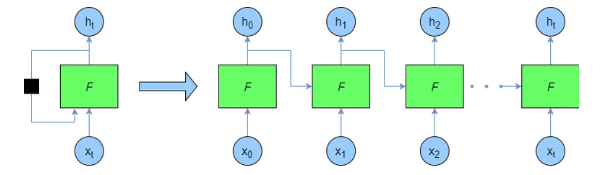
\includegraphics[width=11.5cm , height = 3.5cm]{images/rnn.PNG}

\end{figure}
\end{center}

Training input is time series of features from MD simulation data.
}
%%%%%%%%%%%%%%%%%%%%%%%%%%%%%%%%%%%%%%%%%%%%%%%%%%%%%%%%%%%%%%%%%%%%%%%%%%%%%%%%%%%%%%%%%%%%%%%%%%%%%%%%%%

\frame{
\frametitle{Recurrent Neural Networks}
\begin{block}{}
\begin{itemize}
    \item In training, RNN uses information from all times up to time step $t$, to output feature values and ground truth labels for time $t+1$.
    \begin{itemize}
        \item {\bf Long Short-Term Memory} (LSTM) mechanism gives added weight to information from more recent time steps.
    \end{itemize}
    \item Loss function describes difference between output values and training data.
    \item Neural network weights updated successively, to minimize loss function and improve prediction accuracy.

\end{itemize}
\end{block}
}
%%%%%%%%%%%%%%%%%%%%%%%%%%%%%%%%%%%%%%%%%%%%%%%%%%%%%%%%%%%%%%%%%%%%%%%%%%%%%%%%%%%%%%%%%%%%%%%%%%%%%%%%%%
\frame{
\frametitle{Proposed Architecture}

\begin{center}
\begin{figure}[!b]
    \centering
    \noindent
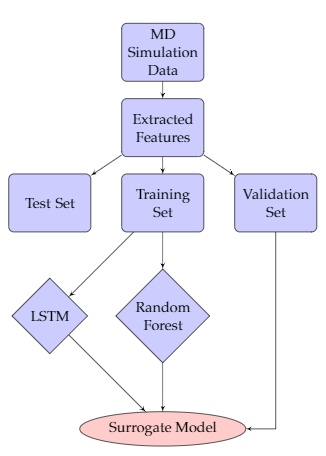
\includegraphics[width=4.5cm , height = 6cm]{images/arch.PNG}

Machine Learning Architecture

\end{figure}
\end{center}

}













%%%%%%%%%%%%%%%%%%%%%%%%%%%%%%%%%%%%%%%%%%%%%%%%%%%%%%%%%%%%%%%%%%%%%%%%%%%%%%%%%%%%%%%%%%%%%%%%%%%%%%%%%%



\section{Status}
\subsection{Some subtitle}
\frame
{
\frametitle{What we have so far}
\begin{block}{}
Here we will talk about what we have discovered so far
\end{block}
}

\subsection{Next Steps}
\frame
{
\frametitle{Next Steps}
\begin{block}{}
Here we will explain our next steps
\end{block}
}
%\section{Bibliography}

\begin{frame}
\frametitle{Bibliography}
\begin{thebibliography}{CGU, 2011}
\bibitem[CGU, 2010]{CGU10}
R. Carrington, and  A. Musselman, and M. Wilson, ``Optimizing Smart Power Grids,'' tech. rep., Claremont Graduate University, 2010-2011.
\bibitem[Silva, 2000]{silva2000}
E. da Silva, H. Gil, and J. Areiza, ``Transmission network expansion planning under an improved genetic algorithm," {\em Power Systems, IEEE Transactions on,} vol. 15, no. 3, pp. 1168–1174, 2000. 
\bibitem[Silva, 2001]{silva2001}
H. Gil and E. Da Silva, ``A reliable approach for solving the transmission network expansion planning problem using genetic algorithms,'' {\em Electric Power Systems Research,} vol. 58, no. 1, pp. 45–51, 2001.
\end{thebibliography}
\end{frame}

\begin{frame}
\frametitle{Bibliography}
\begin{thebibliography}{CGU, 2011}
\bibitem[Djidjev, 2017]{Djidjev-2017}
Djidjev, H., O'Malley, D., Viswanathan, H., Hyman, J., Karra, S., Srinivasan, G., Learning on Graphs for Predictions of Fracture Propagation, Flow and Transport. {\em 2017 IEEE International Parallel and Distributed Processing Symposium Workshops (IPDPSW)}, year={2017}

\bibitem[Boyd, 2008]{boyd2008}
A. Ghosh, S. Boyd, and A. Saberi, ``Minimizing effective resistance of a graph,'' {\em SIAM review,} vol. 50, no. 1, p. 37, 2008.
\bibitem[Boyd, 2008]{boyd2008}
``Map of {C}{A} {C}{R}{E}{Z} Conceptual Transmission Segments Phase 2B Final.'' \url{http://www.energy.ca.gov/reti/documents/phase2B/CA_CREZ_Conceptual_Transmission_Segments_Phase_2B_final.pdf}, 2010.
\end{thebibliography}
\end{frame}



\end{document} 